\section{What  \mixin Generates}\label{sec:translation}

This section shows what the \mixin annotation generates, and presents a
formal definition for most of the generated methods. Since
Classless Java does not consider
% setters, so we do not formally define the generation of the setters.
%We do not include
casts or \Q@instanceof@, the \Q@with@ method is not included in the
formal translation. For the same reason \Q@void@ returning setters are
not included, since they are just a minor variation over the more
interesting fluent setters, and they would require special handling
just for the conventional \Q@void@ type.


\subsection{Translation}

For the purposes of the formalization, the translation is divided in
two parts.  The two parts are important so that we can discuss the
formal properties later. To this aim we introduce the annotation
$\weakAnn$. Its role is only in the translation process, hence is
not part of the Classless Java language.  $\weakAnn$ generates the
constructor method $\QM{of}$, while \mixin automatically refines the
return types and calls $\weakAnn$.


\noindent$\begin{array}{l}
\InTextDef{16em}{[\![\mixinAnn\ \QM{interface}\ \C_0\ \QM{extends}\ \Cs\ \oC \methods\ \cC ]\!]
}{
[\![\weakAnn\ \QM{interface}\ \C_0\ \QM{extends}\ \Cs\ \oC
\methods\ \methods' \cC
]\!]}\\
\InTextWith{\methods'=\otherMethod(\C_0,\methods)}\\

\InTextDef{16em}{[\![\weakAnn\ \QM{interface}\ \C_0\ \QM{extends}\ \Cs\ \oC \methods\ \cC ]\!]
}{
\QM{interface}\ \C_0\ \QM{extends}\ \Cs\ \oC
\methods\ \ofMethod(\C_0) \cC
}\\
\InTextWith{\valid(\C_0),\QM{of}\notin\dom(\C_0) }
\end{array}$

\noindent Note that it is necessary to explicitly check if the interface is valid
for annotation:



\noindent$\begin{array}{ll}
\InTextDef{7ex}{\valid(\C_0)}{\forall \m\in\dom(\C_0),\mbox{ if }\mh\QM; = \mBody(\m, \C_0),\mbox{ one case is satisfied:}}\\
\tab\tab
\isField(\method), \isWith(\method, \C_0) \mbox{ or }
\isSetter(\method,\C_0)\\
\InTextDef{24ex}{\isField(\C\ \m\oR\cR\QM;)}{
\mnot\ \specialName(\m)}\\
\InTextDef{24ex}{\isWith(\C'\ \QM{with#}\m \oR \C\ \x\cR\QM;, \C_0)}{
\C_0 <: \C', \mBody(\m, \C_0) = \C\ \m\oR\cR\QM;
\ \mand\ \mnot\ \specialName(\m)}\\
\InTextDef{24ex}{\isSetter(\C'\ \QM_\m \oR \C\ \x\cR\QM;, \C_0)}{
\C_0 <: \C', \mBody(\m, \C_0) = \C\ \m\oR\cR\QM;
\ \mand\ \mnot\ \specialName(\m)}\\

%\isClone:&\isClone(\C\ \QM{clone}\oR\cR\QM;, \C_0)\tab \mif\ \C_0 <: \C \\
%\isImplemented:&\isImplemented(\method) \tab\mbox{iff }\method\mbox{ not of form }\mh\QM;
%\QM{default}\ \mh\mbox{\Q@\{return \_;\}@}) = \QM{true} \\
%&\isImplemented(\QM{static}\ \mh\mbox{\Q@\{return \_;\}@}) = \QM{true} \\
\end{array}$

\noindent That is, we can categorize all the \emph{not implemented} methods in a pattern that we know how to implement: it is eiter a field getter, a with method or a setter method.

Moreover, we check that the method \Q@of@ is not already defined by the user.
In the formalization an existing definition of the \Q@of@ method is an error. However,
in the prototype (which also needs to account for overloading), the check is more complex
as it just checks that an \Q@of@ method with the same signature of the one being
generated is not already present.


In the following we will write $\QM{with#}\m$ to append $\m$ to
\QM{with}, following the camelCase rule. That is, the first letter of $\m$
must be lower-case and is turned in upper-case upon merging.  For
example \QM{with#foo}=\QM{withFoo}.  Special names $\specialName(\m)$
are \QM{with} and all the identifiers of form $\QM{with#}\m$.

\paragraph{The $\otherMethod$ method:}
The definition of $\otherMethod(\C_0,\methods)$ is as follows:

\noindent$\begin{array}{ll}
\InTextDef{16em}{\C_0\ \QM{with#}\m\oR \C\ \QM{_val}\cR\QM;\in
\otherMethod(\C_0,\methods)}{
 \isWith(\mBody(\QM{with#}\m, \C_0), \C_0)}\\
\hspace{2.65in}{
\mbox{ and } \QM{with#}\m\notin\dom(\methods)}\\
\InTextDef{16em}{\C_0\ \QM_\m\oR \C\ \QM{_val}\cR\QM;\in
\otherMethod(\C_0,\methods)}{\isSetter(\mBody(\QM_\m, \C_0), \C_0),}\\
\hspace{2.65in}{
\mbox{ and } \QM_\m\notin\dom(\methods)}\\
\end{array}$

\noindent The methods generated in the interface are \Q@with-@ and setters. %\Q@clone@.
%A complete formalization would also generate the \Q@with@.
The methods are generated when they are unimplemented in $\C_0$, because
the return types need to be refined.
To discover whether the methods need to be generated,
we check if such \Q@with-@ or setter methods %\Q@clone@
are required by $\C_0$, but are not already present in the methods directly declared in $\C_0$.


\paragraph{The $\ofMethod$ method:}\label{subsec:ofmethod}
The $\ofMethod$ function generates the method
\QM{of}, which behaves like a factory. To avoid boring digressions about
well-known ways to find unique names, for the sake of this formalization we
assume that no-args methods start with an underscore, and we prefix method names with underscore to obtain valid  parameter names.

\noindent$\begin{array}{l}
\InTextDef{5em}{\ofMethod(\C_0)}{
 \QM{static}\ \C_0\ \QM{of} \oR \C_1\ \QM_\m_1\QM,\ldots \C_n\ \QM_\m_n\cR\
\QM{\{}
\QM{return new}\ \C_0 \oR\cR\ \QM{\{} }\\
\tab\tab \C_1\ \m_1 = \QM_\m_1\QM;\ldots \C_n\ \m_n = \QM_\m_n\QM; \\
\tab\tab
\C_1\ \m_1\oR\cR\ \QM{\{return }\ \m_1\QM{;\}}\ \ldots
\C_n\ \m_n\oR\cR\ \QM{\{return }\ \m_n\QM{;\}}\\
\tab\tab\withMethod(\C_1,\m_1,\C_0,\es_1)\ldots\withMethod(\C_n,\m_n,\C_0,\es_n)\\
\tab\tab\setterMethod(\C_1,\m_1,\C_0)\ldots\setterMethod(\C_n,\m_n,\C_0)\\
%\tab\tab\cloneMethod(\C_0,\es)\\
%\tab\tab\withMethod(\C_0)\\
\tab\QM{\};\}} \\
\InTextWith{\fieldsFunc(\C_0)=\C_1\ \m_1\QM{();},\ldots \C_n\ \m_n\QM{();}
\mbox{and }\es_i=\m_1\QM,\ldots\QM, \m_{i-1}\QM,\QM{_val,}\m_{i+1}\QM,\ldots\QM, \m_n}
\end{array}$

\noindent Note that, the function $\fieldsFunc(\C_0)$ denotes all the fields in the current interface:

\noindent$\begin{array}{ll}
\InTextDef{24ex}{\method\in\fieldsFunc(\C_0)}{
\isField(\method)\ \mand\
%}\\\InTextWith{
\method=\mBody(\_,\C_0)
}
\end{array}$

\noindent For methods inside the interface with the form $\C_i\ \m_i$\QM{();}
  \begin{itemize}
   \item $\m_i$ is the field name, and has type $\C_i$.
   \item $\m_i$\QM{()} is the getter, and just returns the current field value.
   \item if a method \Q@with#@$\m_i$ is required, then it is implemented by calling the \Q@of@ method using
    the current value for all the fields except for $\m_i$. Such new value is provided as parameter. This corresponds to the expressions $\es_i$.
\item \QM_$\m_i$\QM($\C_i\ $\QM{ _val)} is the setter. In our prototype we use name $\m_i$, here we use the underscore to avoid modelling overloading.
%   \item similarly, for the \Q@clone@ method, \Q@of@ is called using the current value for all the fields.
   %\item To complete our generation, we need to generate setters, fluent setters and the with method.
   %\item \marco{should we just formalize setters?}
   \end{itemize}

The auxiliary functions are defined below. Note that we do not need to check if some header is a subtype of what we would generate, this is ensured by $\valid(\C_0)$.

\noindent$\begin{array}{l}
\InTextDef{10em}{\withMethod(\C,\m,\C_0,\es)}{
\C_0\ \QM{with#}\m\oR \C\ \QM{_val}\cR\ \QM{\{}
\QM{return}\ \C_0\QM{.of(}\es\QM{);\}}} \\
\InTextWith{\mBody(\QM{with#}\m,\C_0) \mbox{ is of form }\mh\QM;}\\
\InTextDef{10em}{\withMethod(\C,\m,\C_0,\es)}{\emptyset\mbox{ otherwise}}\\
\InTextDef{10em}{\setterMethod(\C,\m,\C_0)}{
\C_0\ \QM_\m\oR \C\ \QM{_val}\cR\ \QM{\{}
 \m\QM{= _val;return this;\}}} \\
\InTextWith{
\mBody(\QM_\m,\C_0) \mbox{ is of form }\mh\QM;}\\
\InTextDef{10em}{\setterMethod(\C,\m,\C_0)}{\emptyset\mbox{ otherwise}}\\
%\cloneMethod:&\cloneMethod(\C_0,\es)=
%\C_0\ \QM{clone()\{return}\ \C_0\QM{.of(}\es\QM{);\}} \\
%&\mbox{iff }
%\mBody(\QM{clone},\C_0) \mbox{ is of form }\mh\QM;\\
%&\cloneMethod(\C_0,\es)=\emptyset\mbox{ otherwise}\\
\end{array}$


\subsection{Other features}

We do not formally model non fluent setters and the \Q@with@ method.
An informal explanation of how those methods are generated is given next:
\begin{itemize}
\item For methods inside the interface with the form \Q@void @$\m$\QM($\C\ \x$\QM{);}:
  \begin{itemize}
    \item Check if method $\C\ \m$\Q@();@ exists. If not, generate error (that is, is not $\valid(\C_0)$).
    \item Generate implemented setter method inside \Q@of@:\\*
           \Q@public void @$\m$\Q@(@$\C$\Q@ _val) { @$\m$\Q@=_val;}@\\*
    Note how there is no need to refine the return type for non fluent setters, thus we do not need to generate the method header in the interface body itself.
    \end{itemize}
\item For methods with the form $\C'\ $\QM{with(}$\C\ \x$\QM{);}:
  \begin{itemize}
   \item $\C$ must be an interface type (no classes or primitive types).
    \item As before, check that $\C'$ is a supertype of the current interface type $\C_0$.
    \item Generate implemented \Q@with@ method inside \Q@of@:\\*
           \Q@public @$\C_0\ $\Q@with(@$\C$\Q@ _val) { @\\*
           \Q@  if(_val instanceof @$\C_0$\Q@){return (@$\C_0$\Q@)_val;}@\\*
${}_{}$\Q@  return @$\C_0$\Q@.of(@$\e_1\ldots\e_n$\Q@);}@\\*
where with $\m_1\ldots\m_n$  fields of $\C_0$,
$\e_i=$\Q@_val.@$\m_i$\Q@()@ if $\C$ has a $\m_i$\Q@()@ method; otherwise
$\e_i=\m_i$.
    \item If needed, as for \Q@with-@ and setters, generate the method header with refined return type in the interface.
 \end{itemize}

%\item For methods with the form $\C'\ \m$\QM($\C\ \x$\QM{);}:
 % \begin{itemize}
  %  \item As for before, check if exist method $\C\ \m$\Q@();@. Also, check that $\C'$ is a supertype of the current interface type $\C_0$.
   % \item Generate implemented setter method inside \Q@of@:\\*
    %       \Q@public @$\C_0\ \m$\Q@(@$\C$\Q@ _val) { @$\m$\Q@=_val; return this;}@
   % \item If needed, as for \Q@with-@ and clone, generate the method header with refined return type in the interface.
 % \end{itemize}
\end{itemize}



\subsection{Guarantees}
To understand to what extent our approach is correct (and more in general, what it means to say that a language tuning is correct) we identify three types of guarantees:

\begin{itemize}
\item \textit{Self coherence}: the generated code itself is well-typed; type errors are not present in code the user have not written.
In our case it means that either \mixin{} produces (in a controlled way) an understandable error, or the class can be successfully annotated and the generated code is well-typed.
We guarantee \textit{Self coherence}.

\item \textit{Client coherence}: all the client code (as for example method calls) that is well-typed without the generation/instrumentation process is well-typed also after the generation.
That is, the annotation does not remove any functionality, is just
adding more behaviour.
We guarantee \textit{Client coherence}.

\item \textit{Heir coherence}: Interfaces (and in general classes) inheriting from instrumented code are well-typed if they were well-typed without the instrumentation.
This would require to not add any (default or abstract) method to the annotated interfaces, including type refinement.
\mixin  does not guarantee \textit{Heir coherence}.
Indeed consider the following:

\begin{lstlisting}
interface A { int x(); A withX(int x); }
@Obj interface B extends A {}
interface C extends B { A withX(int x); }
\end{lstlisting}

\noindent This code is correct before the translation, but \mixin would  generate in \Q@B@  a method ``\Q@B withX(int x);@''.
This would break \Q@C@. \\*
Similarly, an expression of the form ``\Q@new B(){.. A withX(int x){..}}@'' would compile before translation, but would be ill-typed after the translation.
\end{itemize}

\noindent This means that our automatic type refinement
is a useful and convenient feature, but is not transparent to the heirs of the annotated interface. They need to be aware of the annotation semantic  and provide the right type while refining methods.

\subsection{Results}
To formally characterize the behaviour of our annotation, and the two level of guarantees that we offer, we provide some notations and two theorems:
\begin{itemize}
\item We denote with $\C^{\II}$ the name of an interface.
\item An interface table
IT is OK if under such interface table, all interfaces are OK.
\item Since interface tables are just represented as sequences of interfaces we write IT = $\II$ IT' to select a specific interface in a table.
\item IT contains an heir of $\C$ if there is an interface that extends it, or a \Q@new@ that instantiate it.
\end{itemize}


\noindent\textbf{THEOREM }$\weakAnn$ tuning\\*
If a given interface table $\II$ IT is OK
 where $\II$ has $\weakAnn$,
$\valid(\C^{\II})$  and $\QM{of}\notin\dom(\C^{\II})$,
then the interface table $[\![\II]\!]$ IT is OK.

\noindent\textbf{THEOREM }\mixin tuning\\*
If a given interface table $\II$ IT is OK
 where $\II$ has \Q!@Obj!,
$\valid(\C^{\II})$  and $\QM{of}\notin\dom(\C^{\II})$, and there is no heir of $\C^{\II}$,
then the interface table $[\![\II]\!]$ IT is OK.


Informally, the theorems mean that for a client program that
typechecks before a translation is applied, if the annotated type has
no subtypes, and no objects of that type are created, then type safety
is guaranteed after the successful translation. 
 
The second
step of \mixin, namely what $\weakAnn$ does in the formalization, is
guaranteed to be type-safe for the three kinds of coherence by the $\weakAnn$  tuning theorem.  
\mixin
tuning is more interesting: Since \mixin does not guarantee heir
coherence, we exclude explicitly the presence of heirs. In this way
\mixin tuning guarantees only self and client coherence. The formal
theorem proofs are available in the supplementary materials.%~\ref{subsec:lemma1},~\ref{subsec:lemma2} and~\ref{subsec:theorem}.\\





\begin{comment}
\begin{figure}[tbp]
\centering
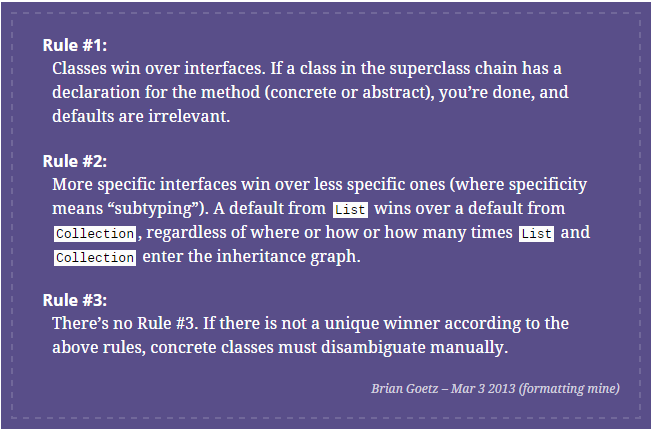
\includegraphics[width=5in]{screenshot.png}
\caption{Screenshot.}\label{screenshot_png}
\end{figure}

\haoyuan{I tried to understand the current algorithm, and did more experiments in eclipse.
Now I borrow some ideas from the current version, and give a new version of the algorithm in text. See below.

(1) I guess the function \textsf{tops} is not necessary. The first step is still
\[\textsf{mbody}(m,C_i)\in\overline{meth}\textrm{ (excluding \textbf{static} methods)}\]

(2) Assume the context is ``interface $C_0$ extends $\overline{C}$ \{$meth'$;...\}''. First handle
\[\textsf{override}(meth',\overline{meth}) \eqno{(*)}\]

(3) If $meth'\ne\none$, $(*)$ returns $meth'$ if
\[\forall meth\in\overline{meth},meth'\subtype meth\]
even if there are conflicts in $\overline{meth}$.

(4) If $meth'=\none$, we need to figure out
\[\textsf{mostSpecific}(\overline{meth})\]
and it should be the one that ``overrides'' all the others in $\overline{meth}$. It means we should not only deal with the return types of methods, but also look into the subtyping relation of interfaces. But for abstract methods, only return types are taken into consideration.
}
\end{comment}

%\text{\yanlin{shouldn't mostSpecific be: $\forall \method' \in \methods : \method \subtype
%  \method'$ ?}}

%(2) If $body_1.\textsf{returnType}=body_2.\textsf{returnType}$, \textsf{shadow} tends to return a default method. If both $body_1$ and $body_2$ are default methods, \textsf{shadow} throws an error.
%\begin{equation*}
%\begin{array}{ll}
%\textsf{shadow}(body_1, body_2)=\textsf{ERROR} & \textsf{if }body_1.\textsf{modifier}=body_2.\textsf{modifier}=\textbf{default}\\
%\textsf{shadow}(body_1, body_2)=body_1 \hspace{.1in} & \textsf{if }body_1.\textsf{modifier}=\textbf{default} \\
%\textsf{shadow}(body_1, body_2)=body_2 \hspace{.1in} & \textsf{if }body_2.\textsf{modifier}=\textbf{default} \\
%\textsf{shadow}(body_1, body_2)=body_1\textsf{ (or }body_2\textsf{)} \hspace{.1in} & \textsf{otherwise}
%\end{array}
%\end{equation*}
%
%(3) If $body_1.\textsf{returnType}<:body_2.\textsf{returnType}$, \textsf{shadow} tends to choose the one with the subtype (namely $body_1$), but only when both methods are abstract, otherwise it gives an error. The other direction $body_2.\textsf{returnType}<:body_1.\textsf{returnType}$ follows the same rule. It also gives an error if there is no subtyping relationship between two return types.
%\begin{equation*}
%\begin{array}{ll}
%\textsf{shadow}(body_1, body_2)=body_1 & \textsf{if }body_1.\textsf{modifier}=body_2.\textsf{modifier}=\emptyset\\
%& \textsf{and }body_1.\textsf{returnType}<:body_2.\textsf{returnType}\\
%\textsf{shadow}(body_1, body_2)=body_2 & \textsf{if }body_1.\textsf{modifier}=body_2.\textsf{modifier}=\emptyset\\
%& \textsf{and }body_2.\textsf{returnType}<:body_1.\textsf{returnType}\\
%\textsf{shadow}(body_1, body_2)=\textsf{ERROR} \hspace{.1in} & \textsf{otherwise}
%\end{array}
%\end{equation*}

%\subsubsection{Auxiliary function: \textsf{replace}}
%
%The \textsf{replace} function takes two same methods (with the same name and types of arguments), and gives the result of the first method overriding the second one.
%
%\begin{equation*}
%\begin{array}{ll}
%\textsf{replace}(body_1, body_2)=body_1 & \textsf{if }body_2=\emptyset\\
%\textsf{replace}(body_1, body_2)=body_2 & \textsf{if }body_1=\emptyset\\
%\textsf{replace}(body_1, body_2)=body_1 & \textsf{if }body_1.\textsf{returnType}<:body_2.\textsf{returnType}\\
%\textsf{replace}(body_1, body_2)=\textsf{ERROR} \hspace{.1in} & \textsf{otherwise}
%\end{array}
%\end{equation*}
